\documentclass{beamer}
\usepackage[utf8]{inputenc}

\usetheme{Madrid}
\usecolortheme{default}
\usepackage{extarrows}
\usepackage{amsmath}
\usepackage{extarrows}
\usepackage{amssymb,amsfonts,amsthm}
\usepackage{txfonts}
\usepackage{tkz-euclide}
\usepackage{listings}
\usepackage{adjustbox}
\usepackage{array}
\usepackage{tabularx}
\usepackage{gvv}
\usepackage{lmodern}
\usepackage{circuitikz}
\usepackage{tikz}
\usepackage{graphicx}
\usepackage{amsmath} 

\setbeamertemplate{page number in head/foot}[totalframenumber]

\usepackage{tcolorbox}
\tcbuselibrary{minted,breakable,xparse,skins}

\definecolor{bg}{gray}{0.95}
\DeclareTCBListing{mintedbox}{O{}m!O{}}{%
  breakable=true,
  listing engine=minted,
  listing only,
  minted language=#2,
  minted style=default,
  minted options={%
    linenos,
    gobble=0,
    breaklines=true,
    breakafter=,,
    fontsize=\small,
    numbersep=8pt,
    #1},
  boxsep=0pt,
  left skip=0pt,
  right skip=0pt,
  left=25pt,
  right=0pt,
  top=3pt,
  bottom=3pt,
  arc=5pt,
  leftrule=0pt,
  rightrule=0pt,
  bottomrule=2pt,
  toprule=2pt,
  colback=bg,
  colframe=orange!70,
  enhanced,
  overlay={%
    \begin{tcbclipinterior}
    \fill[orange!20!white] (frame.south west) rectangle ([xshift=20pt]frame.north west);
    \end{tcbclipinterior}},
  #3,
}
\lstset{
    language=C,
    basicstyle=\ttfamily\small,
    keywordstyle=\color{blue},
    stringstyle=\color{orange},
    commentstyle=\color{green!60!black},
    numbers=left,
    numberstyle=\tiny\color{gray},
    breaklines=true,
    showstringspaces=false,
}
\title %optional
{5.2.35}

\author 
{Kartik Lahoti - EE25BTECH11032}

\begin{document}

\frame{\titlepage}
\begin{frame}{Question}
Solve the following system of linear equations.
\begin{align*}
    3x+4y &= 10
\end{align*}
\begin{align*}
    2x - 2y &= 2
\end{align*}
\end{frame}

\begin{frame}{Theoretical Solution}

The equation of line $L_1$ is,
\begin{align}
    \myvec{3 & 4}\vec{x} = 10
\end{align}
The equation of line $L_2$ is,
\begin{align}
    \myvec{2 & -2}\vec{x} = 2
\end{align}

\end{frame}
\begin{frame}{Theoretical Solution}

On putting the equations in a matrix, we will get
\begin{align}
    \implies \myvec{3 & 4\\2 & -2}\vec{x} = \myvec{10\\2}
\end{align}
So the augmented matrix is,
\begin{align}
    \augvec{2}{1}{3 & 4 & 10\\2 & -2 & 2}
\end{align}
\end{frame}

\begin{frame}{Theoretical Solution}
\begin{align}
     \augvec{2}{1}{3 & 4 & 10\\2 & -2 & 2}\xleftrightarrow[]{R_2\rightarrow R_2-\frac{2}{3}R_1}\augvec{2}{1}{3 & 4 & 10\\0 & \frac{-14}{3} & \frac{-14}{3}}
\end{align}
\begin{align}
    \augvec{2}{1}{3 & 4 & 10\\0 & \frac{-14}{3} & \frac{-14}{3}}\xleftrightarrow[]{R_2\rightarrow \frac{-3}{14}R_2}\augvec{2}{1}{3 & 4 & 10\\0 & 1 & 1}
\end{align}
\begin{align}
    \augvec{2}{1}{3 & 4 & 10\\0 & 1 & 1}\xleftrightarrow[]{R_1\rightarrow R_1-4R_2}\augvec{2}{1}{3 & 0 & 6\\0 & 1 & 1}
\end{align}
\end{frame}

\begin{frame}{Theoretical Solution}

\begin{align}
    \augvec{2}{1}{3 & 0 & 6\\0 & 1 & 1}\xleftrightarrow[]{R_1\rightarrow \frac{1}{3}R_1}\augvec{2}{1}{1 & 0 & 2\\0 & 1 & 1}
\end{align}
\begin{align}
    \implies\vec{x} =\myvec{x\\y}\equiv \myvec{2\\1}
\end{align}
Therefore the two lines will intersect at \myvec{2\\1}.

\end{frame}

\begin{frame}[fragile]
    \frametitle{C Code (1)}

    \begin{lstlisting}
void gaussian(double *A , double *B , double *C , double *X)
{   // works only if all 4 values in A and B are non-zero
    int i = 1 , j = 0 ; 
    if ( A[i] != 0 ){
        B[i] -= A[i]/A[j] * B[j];
        C[i] -= A[i]/A[j] * C[j];
        A[i] = 0 ;}
    if(B[i] != 0){
        C[i]  = C[i] / B[i] ;
        B[i] = 1;}
    if(B[j] != 0){
        C[j] -= C[i] * B[j];
        B[j] = 0 ;}
    X[j] = C[j] / A[j];
    X[i] = C[i];    
}
    \end{lstlisting}
\end{frame}

\begin{frame}[fragile]
    \frametitle{C Code (2) - Function to Generate Points on Line}
    \begin{lstlisting}
void linegen(double *XY, double *A , double *B , int n , int m )
{
    double temp[m] ; 
    for (int i = 0 ; i < m ; i++)
    {
        temp [ i ] = (B[i]- A[i]) /(double) n ; 
    }
    for (int i = 0 ; i < n ; i++ )
        for (int j = 0 ; j < m ; j++)
            XY[j*n + i ] = A[j] + temp[j] * i ; :wq           
}

\end{lstlisting}
\end{frame}

\begin{frame}[fragile]
    \frametitle{Python Code - Using Shared Object}
    \begin{lstlisting}
import ctypes as ct
import numpy as np
import matplotlib.pyplot as plt

handc1 = ct.CDLL("./func.so")

handc1.gaussian.argtypes = [
    ct.POINTER(ct.c_double),
    ct.POINTER(ct.c_double),
    ct.POINTER(ct.c_double),
    ct.POINTER(ct.c_double)
]

handc1.gaussian.restype = None
\end{lstlisting}
\end{frame}

\begin{frame}[fragile]
    \frametitle{Python Code - Using Shared Object}
    \begin{lstlisting}

A = np.array([3,2], dtype = np.float64).reshape(-1,1)
B = np.array([4,-2], dtype = np.float64).reshape(-1,1)
C = np.array([10,2] , dtype = np.float64).reshape(-1,1)
X = np.zeros(2, dtype = np.float64).reshape(-1,1)

handc1.gaussian(
    A.ctypes.data_as(ct.POINTER(ct.c_double)),
    B.ctypes.data_as(ct.POINTER(ct.c_double)),
    C.ctypes.data_as(ct.POINTER(ct.c_double)),
    X.ctypes.data_as(ct.POINTER(ct.c_double)),
)
print("Vector X = " , X)

\end{lstlisting}
\end{frame}

\begin{frame}[fragile]
    \frametitle{Python Code - Using Shared Object}
    \begin{lstlisting}
def line(P: np.ndarray , Q: np.ndarray, str1 , str2):
    handc2 = ct.CDLL("./line_gen.so")

    handc2.linegen.argtypes = [
        ct.POINTER(ct.c_double),
        ct.POINTER(ct.c_double),
        ct.POINTER(ct.c_double),
        ct.c_int , ct.c_int
    ]

    handc2.linegen.restype = None

    handc2.line_cre.restype = None
\end{lstlisting}
\end{frame}
\begin{frame}[fragile]
    \frametitle{Python Code - Using Shared Object}
    \begin{lstlisting}
n = 200
    XY = np.zeros((2,n),dtype=np.float64)

    handc2.linegen (
        XY.ctypes.data_as(ct.POINTER(ct.c_double)),
        P.ctypes.data_as(ct.POINTER(ct.c_double)),
        Q.ctypes.data_as(ct.POINTER(ct.c_double)),
        n,2
    )
    plt.plot(XY[0,:],XY[1,:], str1 , label = str2 )
    \end{lstlisting}
\end{frame}

\begin{frame}[fragile]
    \frametitle{Python Code - Using Shared Object}
    \begin{lstlisting}

P = np.array([6,-2], dtype = np.float64).reshape(-1,1)
Q = np.array([-6,7], dtype = np.float64).reshape(-1,1)
line(P,Q,"g-"," Line 1 ")
P = np.array([8,7], dtype = np.float64).reshape(-1,1)
Q = np.array([-8,-9], dtype = np.float64).reshape(-1,1)
line(P,Q,"r-"," Line 2 ")
plt.scatter(X[0,0], X[1,0])
plt.annotate(f"X\n({X[0,0]},{X[1,0]})",
                    (X[0], X[1]),
                    textcoords = "offset points" ,
                    xytext = (0,12),ha = "center")

\end{lstlisting}
\end{frame}

\begin{frame}[fragile]
    \frametitle{Python Code - Using Shared Object}
    \begin{lstlisting}

plt.xlim([-1,4])
plt.ylim([-1,4])
plt.xlabel("$x$")
plt.ylabel("$y$")
plt.grid()
plt.legend(loc="best")
plt.title("5.2.35")
plt.savefig("../figs/intersect1.png")
plt.show()
#plt.savefig('../figs/intersect1.png')
#subprocess.run(shlex.split("termux-open ../figs/intersect1.png"))


\end{lstlisting}
\end{frame}

\begin{frame}[fragile]
    \frametitle{Python Code}
    \begin{lstlisting}
import math
import sys 
sys.path.insert(0, '/home/kartik-lahoti/matgeo/codes/CoordGeo')
import numpy as np
import numpy.linalg as LA
import matplotlib.pyplot as plt

from line.funcs import *

#if using termux
#import subprocess
#import shlex
\end{lstlisting}
\end{frame}

\begin{frame}[fragile]
    \frametitle{Python Code }
    \begin{lstlisting}

A = np.array([[3,4],
              [2,-2]], dtype = np.float64)
C = np.array([10,2] , dtype = np.float64).reshape(-1,1)

X = LA.solve(A,C)
print("Vector X = " , X ) 

def plot_it(P,Q,str1,str2):
    x_l = line_gen_num(P,Q,20)
    plt.plot(x_l[0,:],x_l[1,:] , str1 , label =  str2)

\end{lstlisting}
\end{frame}

\begin{frame}[fragile]
    \frametitle{Python Code }
    \begin{lstlisting}
plt.figure()
P = np.array([6,-2], dtype = np.float64).reshape(-1,1)
Q = np.array([-6,7], dtype = np.float64).reshape(-1,1)
plot_it(P,Q,"g-"," Line 1 ")
P = np.array([8,7], dtype = np.float64).reshape(-1,1)
Q = np.array([-8,-9], dtype = np.float64).reshape(-1,1)
plot_it(P,Q,"r-"," Line 2 ")
plt.scatter(X[0,0], X[1,0])
plt.annotate(f"X\n({X[0,0]},{X[1,0]})",
                    (X[0], X[1]),
                    textcoords = "offset points" ,
                    xytext = (0,12),ha = "center")
\end{lstlisting}
\end{frame}

\begin{frame}[fragile]
    \frametitle{Python Code }
    \begin{lstlisting}

plt.xlim([-1,4])
plt.ylim([-1,4])
plt.xlabel("$x$")
plt.ylabel("$y$")
plt.grid()

plt.legend(loc="best")

plt.title("5.2.35")

plt.savefig("../figs/intersect2.png")
plt.show()

#plt.savefig('../figs/intersect2.png')
#subprocess.run(shlex.split("termux-open ../figs/intersect2.png"))

    \end{lstlisting}
\end{frame}

\begin{frame}{Plot}
    \centering
    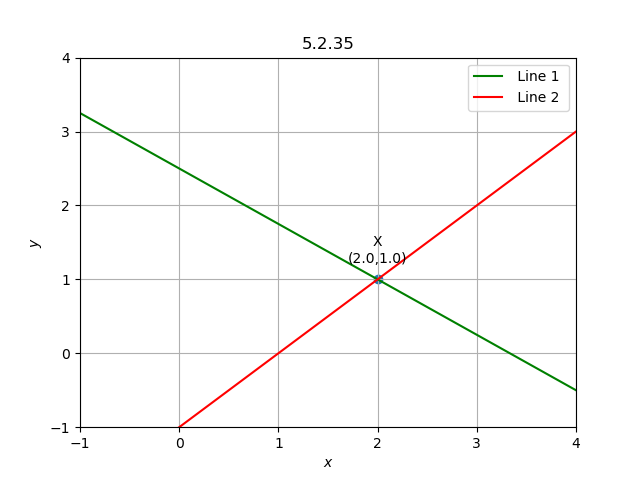
\includegraphics[width=\columnwidth, height=0.8\textheight, keepaspectratio]{../figs/intersect1.png}   
\end{frame}


\end{document}
